\documentclass[11pt]{article}
\usepackage{preamble}
\usepackage{import}
\usepackage{csquotes}
\usepackage{makeidx}
\usepackage{bookmark}
%\usepackage[backend=biber]{biblatex}    % , sorting=none, style=phys
%\addbibresource{refs.bib}

\usepackage{cite}


\title{Quantum chaos}
\author{V}
\date{2025}

\begin{document}
\maketitle
\section{Introduction}
We want to understand quantum chaos, where chaos manifest itself in the statistical properties of our system.
To do this, let us consider a quantum system whose classical counterpart is chaotic: the quantum billiard. 

\section{Quantum rectangular billiard}
Let us start from the simplest geometry: the rectangle, that is we want to solve the Helmholtz equation 
\begin{equation}
    -\nabla^2 \psi = E_n \psi, \quad \nabla = \left(\frac{\partial^2}{\partial x^2} + \frac{\partial^2}{\partial y^2}\right),
\end{equation}
on a rectangular domain $\Omega$ of size $L_x \times L_y$ and Dirichlet boundary conditions $\psi|_{\partial \Omega} = 0$. 
We can then compare the numerical eigenvalues found with the analytical solution Fig.~\ref{fig:energy_comparison}
\begin{equation}
    E_{n,m} = \pi^2(\frac{n^2}{L_x^2} + \frac{m^2}{L_y^2}), \quad n,m \in \mathbb{N}.
\end{equation}
\begin{figure}[h]
    \centering
    \includegraphics[width=0.5\textwidth]{../figs/rect_energy_comparison_100.png}
    \caption{Comparison between numerical and analytical eigenvalues for the rectangular billiard. The red line is $y=x$.}
    \label{fig:energy_comparison}
\end{figure}
To perform the numerical computation, we first discretize the domain and then we build the Hamiltonian matrix corresponding to the Laplacian operator using finite differences: we start from the $1D$ Laplacian with step $h$
\begin{equation}
    u^{''}_i = \frac{u_{i+1} - 2u_i + u_{i - 1}}{h^2}
\end{equation} 
from which we can build the tridiagonal matrix
\begin{equation}
    A = \frac{1}{h^2} \begin{pmatrix}
        -2 & 1 & 0 & \cdots & 0 \\
        1 & -2 & 1 & \cdots & 0 \\
        0 & 1 & -2 & \cdots & 0 \\
        \vdots & \vdots & \vdots & \ddots & \vdots \\
        0 & 0 & 0 & \cdots & -2
    \end{pmatrix}.
\end{equation}
Then we obtain the $2D$ Laplacian using the Kronecker product
\begin{equation}
    \nabla^2= A_x \otimes I_y + I_x \otimes A_y,
\end{equation}
where $I$ is the identity matrix of appropriate size. Finally, the Hamiltonian is given by $H = -\nabla^2$.

\section{The Expansion method}
Now we want to generalize our approach to different geometries, for example the Bunimovich stadium. 
To do this, we will introduce a more general method, called the Expansion method (EM) \cite{10.1119/1.19208}, 
to construct the Hamiltonian that we want to diagonalize.
The idea is to start from the rectangular billiard $L_x \times L_y$, of which we know the eigenvalues $E_{n, m}$ and the eigenfunctions $\phi_{n, m}(x)$, which circumscribe our domain $\Omega$.
\begin{figure}[h]
    \centering
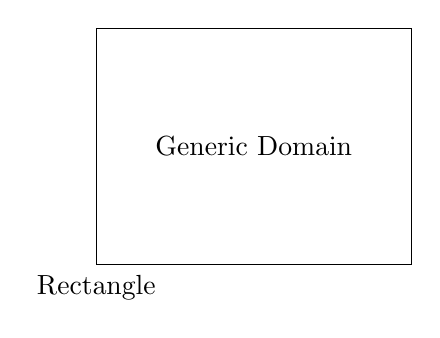
\begin{tikzpicture}
    % Draw the rectangle
    \draw (0,0) rectangle (4,3);

    % Calculate the center and radius of the circle that fits inside the rectangle
    \def\rectWidth{4}
    \def\rectHeight{3}
    \def\circleRadius{\min(\rectWidth/2, \rectHeight/2)}

    % Draw the generic domain (circle) inside the rectangle
    %\draw[thick, blue] (\rectWidth/2 - \circleRadius, \rectHeight/2 - \circleRadius) rectangle (\rectWidth/2 + \circleRadius, \rectHeight/2 + \circleRadius);

    % Add labels if needed
    \node at (0,-0.3) {Rectangle};
    \node at (2,1.5) {Generic Domain};

\end{tikzpicture}
\end{figure}
The 
\begin{equation}
    \phi_{n,m} = \sqrt{\frac{2}{L_x}} \sin\left(\frac{\pi}{L_x} n x\right) \sqrt{\frac{2}{L_y}} \sin\left(\frac{\pi}{L_y} m y\right)
\end{equation}
are an orthonormal basis:
\begin{equation}
    \int_{\text{Rect}}dx\, \phi_{n,m}(x) \phi_{h, k}(x) = \delta_{n, h}\delta_{m, h},
\end{equation}
that is we can expand any function $\psi(x)$ as 
\begin{equation}
    \psi(x) = \sum_{n, m} c_{n, m}\phi_{n,m}.
\end{equation}
Let us now change the notation so to simplify it: instead of using two indices $n,m$ from $1$ to $N$, we will use a single index $i$ from $1$ to $N^2$. 
The expansion of $\psi$ then reads
\begin{equation}
    \psi(x) = \sum_i c_i \phi_i(x).
    \label{eq:em_psi}
\end{equation}
Suppose now $\psi(x)$ satisfies the Schrödinger equation over the domain $\Omega$
\begin{equation}
    H \psi = E \psi, 
\end{equation}
where the Hamiltonian $H$ is the Laplacian plus the potential
\begin{equation}
    V(x) = \begin{cases}
        0,& x \in \Omega \\
        \infty,& \text{otherwise}.
    \end{cases}
\end{equation}
It is useful in this problem to slightly change the potential in the following way
\begin{equation}
    V(x) = \begin{cases}
        0,& x \in \Omega \\
        V_0 (\gg \max\{E_n\}),& x \in \text{Rect} \setminus \Omega\\
        \infty,& \text{otherwise}.
    \end{cases}
\end{equation}
The region $\text{Rect} \setminus \Omega$ will also be called region II.\\
Substituting \eqref{eq:em_psi} we get 
\begin{equation}
    \sum_{ij} \left(H_{ij} - E \delta_{ij}\right) c_j = 0,
\end{equation}
where
\begin{equation}
    H_{ij} = \int_{\text{Rect}}dx\, \phi_{i}(x) H \phi_{j}(x) = E_{ij} \delta_{ij} + V_0 v_{ij},
\end{equation}
and 
\begin{equation}
    v_{ij} = \int_{\text{II}}dx\, \phi_{i}(x) \phi_{j}(x).
\end{equation}
So now the problem is to diagonalize the Hamiltonian.

\section{The Bunimovich Stadium}
Section to define the Bunimovich Stadium. Work in progress...

\section{Results for the Stadium}

\bibliography{refs.bib}{}
\bibliographystyle{ieeetr}
\end{document}